\chapter{Nuclear Shape Deformations}

Rick Casten has given several lectures about nuclear shape deformations and other such things. A lot of this will probably just be restating things he has said in my own words.

First of all, one important tool that you should understand in order to talk about nuclear shape deformations is a Nilsson diagram. First of all, you've seen level diagrams in atomic and nuclear spectroscopy. Figure \ref{fig:NuclearShells}, for instance, is a familiar illustration of low-lying energy levels for a harmonic oscillator potential, both before and after adding a spin-orbit interaction term which leads to the well-known nuclear "magic numbers."

\begin{wrapfigure}{R}{0.5\textwidth}
%\centering
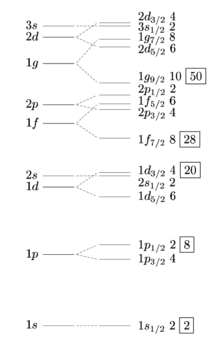
\includegraphics[width=0.45\textwidth]{TeX_files/NuclearShells}
\caption[Nuclear Shell Model level diagram]{From Wikipedia: "Low-lying energy levels in a single-particle shell model with an oscillator potential (with a small negative l2 term) without spin-orbit (left) and with spin-orbit (right) interaction. The number to the right of a level indicates its degeneracy, (2j+1). The boxed integers indicate the magic numbers."}
\label{fig:NuclearShells}
\end{wrapfigure}

Now imagine you stretch out the nucleus somehow. That'll certainly change the spacing and position of the energy levels, because some electron orbitals have a sort of intrinsic shape characteristic that might be better- or worse-suited for the new elongation.

Finally, imagine that you do the stretching \textit{continuously}. That is what is done in a Nilsson diagram. For example, in figure \ref{fig:NilssonDiagram}, the system is elongated from a spherical ground state, and the changing energy levels are the curves, which frequently end up crossing one another. An important thing to notice is that, for different deformations you might have different shell gaps, and as well you might find that different orbitals are more favorable at different deformations.

\begin{figure}
\centering
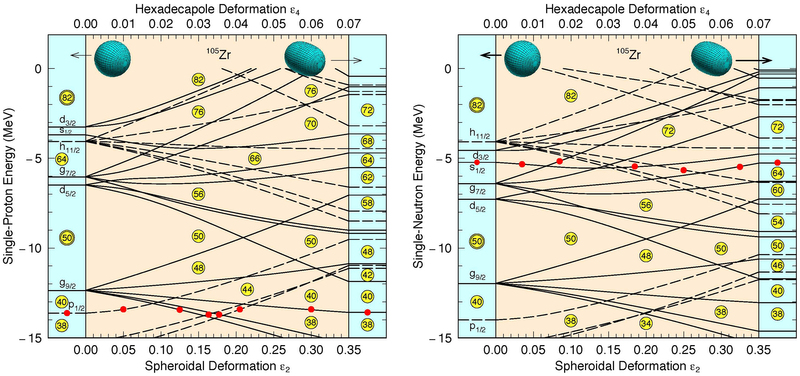
\includegraphics[width=0.7\linewidth]{TeX_files/NilssonDiagram}
\caption[Nilsson Diagram for Zr-105]{Nilsson Diagram for Zr-105, plotted against elongation parameter $\epsilon_2$}
\label{fig:NilssonDiagram}
\end{figure}

Anyway, that's all helpful \textit{once you know} the deformation. And there's a lot of useful and interesting things you can say and predict using a Nilsson diagram - heck, if you know the shape you can [qualitatively] even \textit{draw} a Nilsson diagram, just by thinking about the physical system and how the orbitals are probably behaving.  BUT if you want to understand why a nucleus deforms in the first place, that's a whole other story.

\section{What causes nuclear ground state deformations?}

As with most peculiarities of nuclear structure, the source of nuclear deformation is primarily an artifact of shell structure. In particular, when there is a large shell gap, the nucleus will get sort of "locked" into a particular stable configuration, and if that happens to be a deformed configuration because of the orbital characteristics of the outermost nucleons (because that's the only thing that could matter, right?), then so be it.

A question that I have is how is there ground state deformation in even-even nuclei? Because even-even nuclei all have, without exception, spin-parity $0^+$, and yet $^{152}Dy$ (for example) is highly-deformed. Am I misunderstanding the implications of such a spin-parity assignment? Or am I misunderstanding what is meant by "ground state deformed"?

I don't think this is a real answer, but one way to identify even-even deformed nuclei is to look for nuclei with a large $\frac{E(4^+)}{E(2^+)}$ ratio (or a related method is to look for those with a relatively-small $E(2^+)$).

\section{Phenomenology of Nilsson Diagrams}

[Basically here is where you were thinking about Casten's slides. He goes through and talks about whether a level's energy will go up or down, and how it will curve, just by thinking about the orbital motion of single particles around different axes of the deformed system.]